%%% Local Variables:
%%% mode: latex
%%% TeX-master: "../doc"
%%% coding: utf-8
%%% End:
% !TEX TS-program = pdflatexmk
% !TEX encoding = UTF-8 Unicode
% !TEX root = ../doc.tex
\section{Das Web}
Im folgenden wird der Begriff "Das Web" vereinfacht für die Plattform von verschiedenen Web Technologien genutzt. Dies beinhaltet insbesondere vom W3C veröffentlichte Spezifikationen.

\section{3D-Rendering im Web}
3D-Visualisierungen werden in vielen Branchen verwendet.
So sind zum Beispiel im medizinischen Bereich 3D Scans hilfreich bei der Analyse von Verletzungen.
Für Normalbenutzer ist wohl die Spieleindustrie ein bekanntes Beispiel.
In vielen weiteren Bereichen sind dank leistungsstärkeren Geräten auch realere und somit komplexere Visualisierungen möglich. 

Viele Anwendungen sind auf spezifische Hardware wie zum Beispiel die Spielkonsolen PlayStation oder Xbox angewiesen.

Für hardwareunabhängige Anwendungen eignet sich das Web hervorragend. Viele Benutzer haben Zugang zu einem Desktop, Tablet oder Mobiltelefon.
Somit ermöglicht das Web Anwendungen mit weniger Aufwand einer grösseren Masse zugänglich zu machen.
Heutzutage ist es auch möglich, komplexe 3D Visualisierungen im Web zu realisieren.
Als Basis dafür dient meist das von der Khronos Group entwickelte WebGL, das von allen modernen Browsern unterstützt wird.
Alternativ zu WebGL wird zurzeit ein weiterer Standard entwickelt: WebGPU.
Dieser ist zur Zeit des Schreibens noch in Entwicklung und wird deshalb nicht weiter berücksichtigt, auch wenn ein grosses Potenzial vorhanden ist.

Die Unabhängigkeit der Hardware bedeutet jedoch auch, dass Optimierung der Performanz in Webanwendungen unabdinglich ist, um allen Benutzern ein optimales Erlebnis zu ermöglichen.
Im Vergleich zu fixen Hardware Anwendungen ist es realistisch, dass eine Web Anwendung sowohl auf einem leistungsfähigen Desktop Computer als auch auf einem günstigen Mobilgerät verwendet wird.

Zudem ist WebGL eine junge Technologie und wurde erst 2011 veröffentlicht – verglichen mit dem initialen Release Date von OpenGL welches im Jahre 1992 publiziert wurde.
Nicht nur das Alter, sondern auch die Natur der Web Plattform haben dazu beigetragen, dass WebGL ein langsames Wachstum zu Beginn verspürt hat. Um einen Webstandard wie WebGL einsetzen zu können müssen alle grossen Browser die Spezifikation implementieren. So hat zum Beispiel Internet Explorer 10 keinen Support und es wurde erstmals Ende 2013 möglich im Internet Explorer 11 3D Anwendungen für ein breites Publikum zu entwickeln.

\section{3D-Modelle}
Ein Modell stellt ein Objekt aus der realen Welt vereinfacht dar.
3D-Modelle können vereinfacht als Gruppe von Punkten definiert werden.
Um im dreidimensionalen Raum Objekte visualisieren zu können sind mindestens drei Punkte notwendig.
Punkte von 3D Modellen werden im folgenden als Vertex (Eckpunkte) bezeichnet und können als Vektor definiert werden.
So können wir einen Vertex am Ursprung eines Koordinatensystems definieren als:
$$ V =
\begin{bmatrix}
  0 \\
  0 \\
  0
\end{bmatrix}
$$
Eine Sammlung von drei Vertices bildet ein Dreieck. Um komplexere Formen wie Vierecke (Quads) zu bilden werden jeweils Dreiecke kombiniert.
Für eine Sammlung von Punkten wird generell der Term Polygon verwendet.
Ein Modell besteht aus einer beliebigen Anzahl Polygone.
Polygone bestehen aus einer theoretisch beliebigen Anzahl Vertices.

Die Verbindung zwischen zwei Vertices ist eine sogenannte Edge (Kante).
Verbindet man die Punkte eines Polygons und füllt die Fläche, ergibt sich schlussendlich ein Face (Fläche).

\paragraph{Visuelle Attribute}
Neben den geometrischen Attributen verfügt ein Modell ebenfalls über visuelle Attribute.

So wird für jeden Vertex ein sogenannter Normal definiert. Ein Normal ist ein Vektor der im einfachsten Fall perpendikular zu den zwei an diesem Vertex verbundenen Edges verläuft. Normals werden häufig für das Berechnen von Reflexionen verwendet.
Normals werden auch für Performanz Optimierungen eingesetzt, dazu mehr in \autoref{chap:backfaceCulling}.

Um die Oberfläche von Modellen zu definieren wird häufig ein sogenanntes Texture Mapping durchgeführt. Hierfür sind zusätzliche Informationen für ein Modell notwendig. In der Praxis finden viele weitere Methoden Anwendung, auf diese wird jedoch hier nicht weiter eingegangen.

\section{Transformation von Modellen}

Um ein Modell vereinfachen zu können muss es verändert werden.
Diese Veränderungen können in Basis Operationen vereinfacht erläutert werden.

Im Folgenden werden Transformationen mithilfe einer 2D Visualisierung erläutert. Das Modell könnte jedoch ebenfalls im dreidimensionalen Raum sein - die funktionsweise bleibt identisch.

Für die folgenden Beispiele wird jeweils das Modell aus Abbildung \ref{fig:transformationOriginal} verwendet.

\begin{figure}[H]
  \centering
  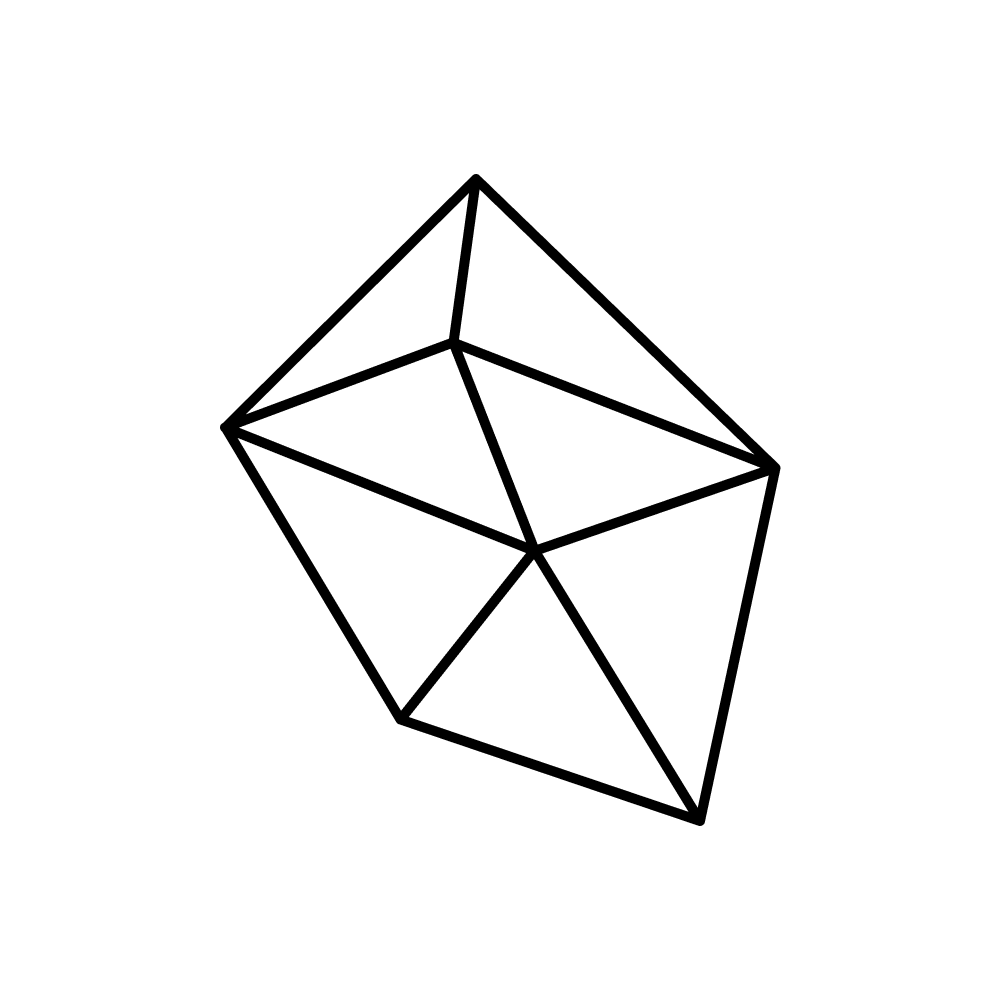
\includegraphics[width=0.4\columnwidth]{grundlagen/transformationen/original.png}
  \caption{Modell Basis}
  \label{fig:transformationOriginal}
\end{figure}

\paragraph{Edge Collapse}
Hierbei werden zwei nebeneinanderliegende Vertices kombiniert, siehe Abbildung \ref{fig:transformationEdgeCollapse}.
Die Umkehrfunktion nennt man Vertex Split.

\begin{figure}[H]
  \centering
  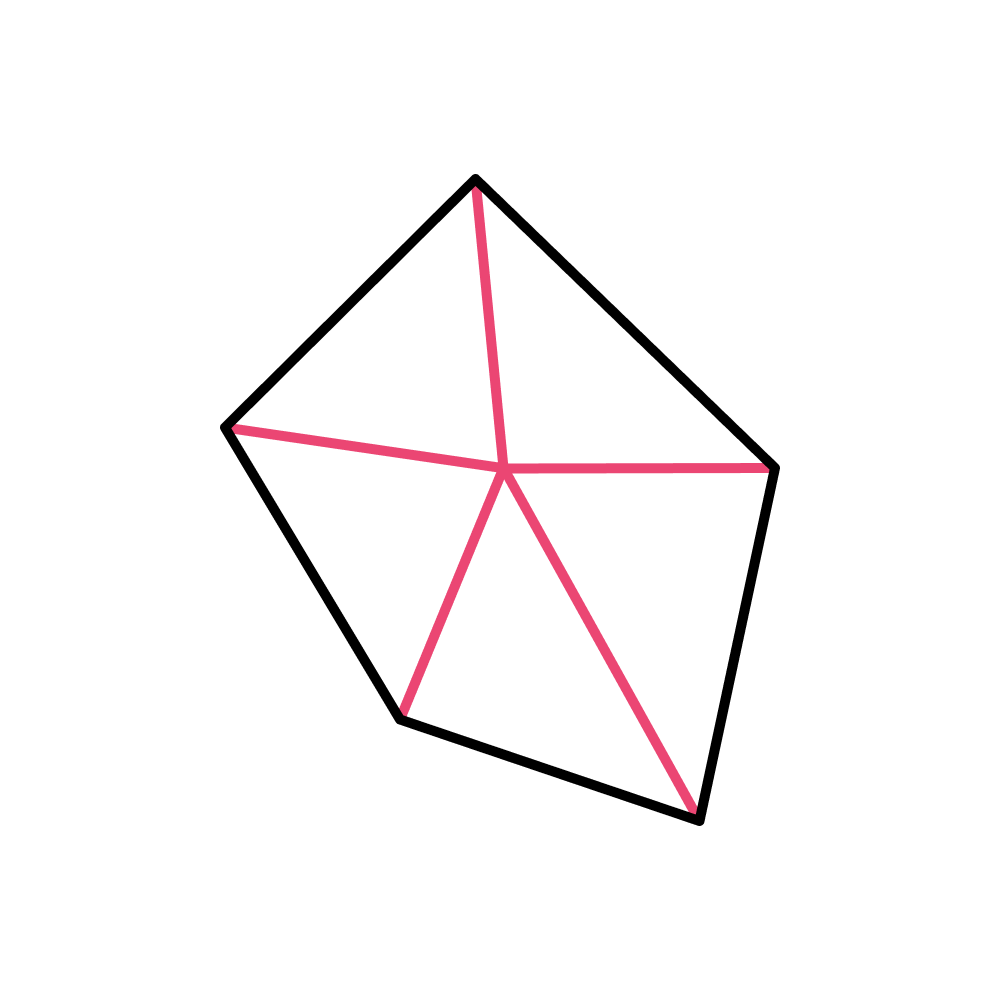
\includegraphics[width=0.4\columnwidth]{grundlagen/transformationen/edge-collapse.png}
  \caption{Edge Collapse}
  \label{fig:transformationEdgeCollapse}
\end{figure}

\paragraph{Halfedge Collapse}
Hierbei wird ein Vertex direkt entfernt und alle Edges auf einen danebenliegenden Vertex zusammengelegt, siehe Abbildung \ref{fig:transformationHalfedgeCollapse}.

\begin{figure}[H]
  \centering
  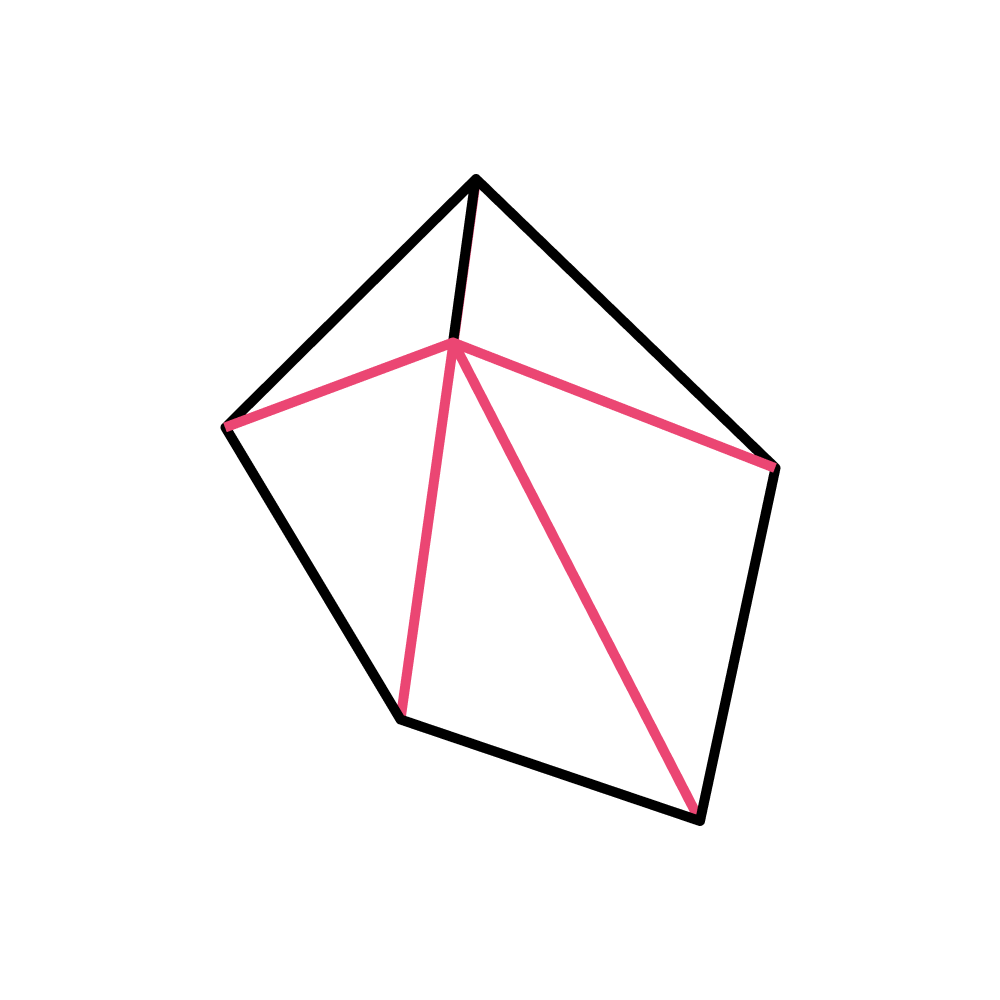
\includegraphics[width=0.4\columnwidth]{grundlagen/transformationen/half-edge-collapse.png}
  \caption{Halfedge Collapse}
  \label{fig:transformationHalfedgeCollapse}
\end{figure}

\paragraph{Vertex Removal}
Hierbei wird ein Vertex entfernt und das Resultat neu trianguliert.
In Abbildung \ref{fig:transformationVertexRemovalOriginal} wird der zentrale Vertex entfernt. Der neu triangulierte Polygon ist in Abbildung \ref{fig:transformationVertexRemovalFinal} ersichtlich.

\begin{figure}[H]
  \centering
  \begin{minipage}{.5\textwidth}
    \centering
    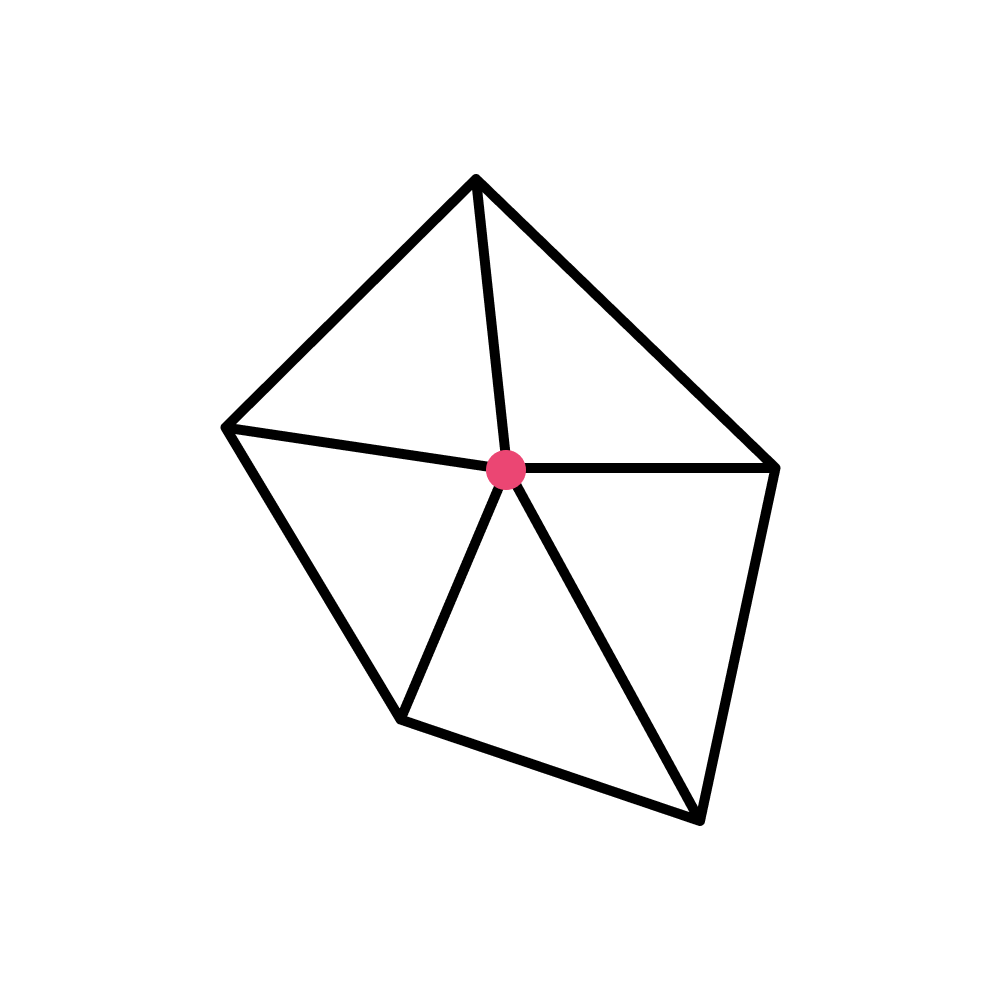
\includegraphics[width=.4\linewidth]{grundlagen/transformationen/vertex-removal-original.png}
    \captionof{figure}{Vertex Removal Ausgangslage}
    \label{fig:transformationVertexRemovalOriginal}
  \end{minipage}
  \begin{minipage}{.5\textwidth}
    \centering
    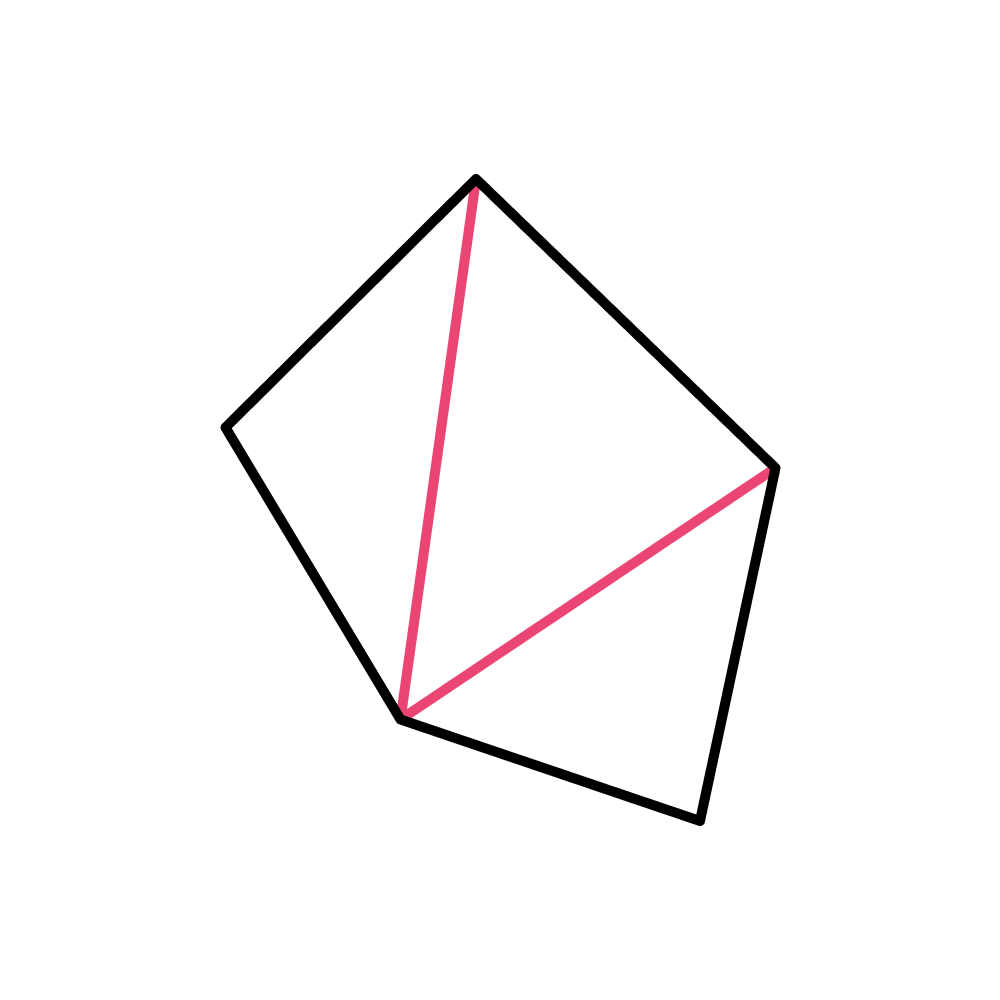
\includegraphics[width=.4\linewidth]{grundlagen/transformationen/vertex-removal-final.png}
    \captionof{figure}{Vertex Removal Resultat}
    \label{fig:transformationVertexRemovalFinal}
  \end{minipage}
\end{figure}

\section{Einführung LOD}
Als Level Of Detail (LOD) werden die verschiedenen Detailstufen bei der virtuellen Darstellung bezeichnet.
Dies wird verwendet, um die Geschwindigkeit von Anwendungen zu steigern, indem Objekte im Nahbereich detailiert angezeigt werden; wohingegen Elemente im Fernbereich deutlich vereinfacht dargestellt werden.

\subsection{Das Problem}
Geometrische Objekte können zu Komplex werden, um jederzeit performant und interaktiv gerendert zu werden.
Gerade wenn viele Objekte zur selben Zeit sichtbar sind, lohnt es sich, zu priorisieren und gewisse Objekte in reduzierter Qualität anzuzeigen.
Im Idealfall geschieht dies jedoch, ohne dass der Anwender dies bemerkt.

\subsection{Lösungsansätze}
In diesem Abschnitt werden mögliche Ansätze erklärt, welche helfen sollen, die Render-Perfomanz zu erhöhen. Diese Arbeit konzentriert sich jedoch auf den Ansatz von Level of Detail; die anderen Ansätze werden nur kurz erläutert.

\paragraph{Level of Detail}
Level of Detail auch bekannt als polygonale Simplifizierung, geometrische Simplifizierung oder Mesh Reduzierung basiert darauf, die Komplexität von Objekten zu reduzieren, welche weiter von der Kamera entfernt werden. Es gibt verschiedene Ansätze zur Generierung von LODs, welche in Abschnitt XY im Detail erläutert werden. Zudem braucht es einen berechenbare Methode, die Genauigkeit von Modellen zu definieren, um diese entsprechend anzuwenden. Schlussendlich ist dann noch zu definieren, ab wann welche Artefakte verwendet werden soll, basierend auf der Genauigkeit und der Komplexität.

\begin{figure}[H]
\centering
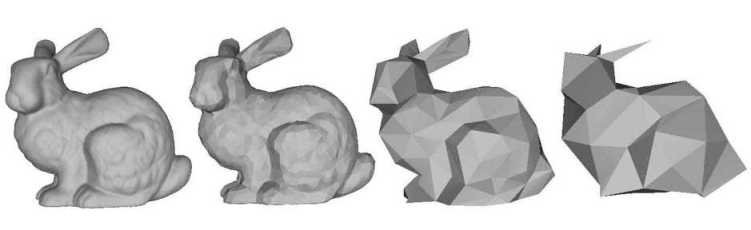
\includegraphics[width=0.8\columnwidth]{LODs-of-a-bunny-model-Courtesy-Stanford-3D-Scanning-Repository-From-left-to-right}
\caption{Level Of Detail Visualisierung vier Hasen}
\label{fig:LevelOfDetailVisualisierungvierHasen}
\end{figure}

Wie in der Abbildung \ref{fig:LevelOfDetailVisualisierungvierHasen} zu erkennen ist, wird von links nach rechts der Detailgrad und somit die Komplexität des Objektes reduziert. Sind es im Bild ganz links noch 69'451 Polygone, wird es bereits im ersten Schritt auf 2'502 Polygone reduziert. Dies ist eine enorme Reduktion von ca 96.5\%. Im dritten Schritt wird die Anzahl Polygone wiederum um ca. 90\% auf 251 reduziert. Schlussendlich hat das letzte Objekt noch 76 Polygone was knapp 0.1\% der ursprünglichen Anzahl entspricht.

\paragraph{Parallel rendering}
Lorem ipsum

\paragraph{Frustum culling}
Polygone, welche nicht im Kamera Frustum enthalten sind, werden bei dieser Methode nicht weiter prozessiert.
Dies reduziert die Anzahl Polygone drastisch.

\paragraph{Occlusion culling}
Polygone bzw. Objekte, welche komplett von anderen Objekten überdeckt werden, werden bei dieser Variante nicht prozessiert.

\paragraph{Backface culling}
\label{chap:backfaceCulling}
Bei dieser Methode wird berechnet welche Polygone zur Kamera orientiert sind.
Alle Polygone, welche in die andere Richtung zeigen werden nicht gezeichnet.
Dies ist nicht immer gewünscht, für die meisten Anwendungen ist diese Optimierung jedoch aktiviert.
Als Grundlage für die Berechnung werden die Normals der Vertices berücksichtigt.

\paragraph{Image-based rendering}
Lorem ipsum


\subsection{Verschiedene Ansätze zur Generierung von LOD Modellen}
Es gibt verschiedene Ansätze, 3D-Modelle mittels LOD zu vereinfachen. In diesem Abschnitt werden einige davon detaillierter erläutert so wie ihre Vor- und Nachteile aufgezeigt.

\paragraph{Diskrete LOD (DLOD)}
Bei diskreten LOD werden für ein detailliertes Modell mehrere weniger detaillierte Modelle verwendet.
Abhängig von der Distanz zum Betrachter wird das optimale Modell gewählt.
\begin{itemize}
  \pro Simplizität: Keine Anpassungen am Scene Graph notwendig
  \con Harte Grenzen: Veränderung des Objektes kann merkbar sein
  \con Kein Clustering möglich: Probleme bei sehr grossen oder vielen kleinen Modellen
\end{itemize}

\paragraph{Kontinuierliche LOD (CLOD)}
Im Gegensatz zu DLOD wird bei CLOD vereinfachende Veränderungen an einem Modell gespeichert.
\begin{itemize}
  \pro Weiche Grenzen: Interpolation zwischen Auflösungen ist möglich
  \con Runtime Performance
  \con Kein Clustering möglich
\end{itemize}

\paragraph{Hierarchische LOD (HLOD)}
Bei HLOD werden mehrere Objekte in einen Cluster gruppiert.
\begin{itemize}
  \pro Clustering möglich
\end{itemize}
